%%%%%%%%%%%%%%%%%%%%%%%%%%%%%%%%%%%%%%%%%%%%%%%%%%%%%%%%%%%%%%%%%%%%%%%
%%% 
%%%    formats1.tex
%%%
%%%    A short description of the data formats 
%%%    involved in the MC simulation
%%%
%%%    J.C. Gonzalez 
%%%
%%%    Dpto.Fisica Atomica, Molecular y Nuclear
%%%    Facultad CC. Fisicas, UCM
%%%    Avda.Complutense s/n
%%%    E-28040 Madrid, Spain
%%%
%%%-----------------------------------------------------------------
%%%  Kopyleft (K) 2000 J C Gonzalez
%%%  Max-Planck-Institut fuer Physik, 
%%%  Foehringer Ring 6, 80805 Muenchen, Germany
%%%  E-mail: gonzalez@mppmu.mpg.de
%%%-----------------------------------------------------------------
%%%  This program is free software; you can redistribute, copy,
%%%  modify, use it and its documentation for any purpose,
%%%  provided that the above copyright notice appear in all
%%%  copies and that both that copyright notice and this
%%%  permission notice appear in supporting documentation.
%%%  
%%%  This piece of code is distributed in the hope that it will
%%%  be useful, but WITHOUT ANY WARRANTY; without even the
%%%  implied warranty of FITNESS FOR A PARTICULAR PURPOSE.
%%%
%%%  Although you can actually do whatever you want with this
%%%  file (following the copyright notice above), your are 
%%%  strongly encouraged NOT to edit directly this file. 
%%%  Instead, make a copy and edit the copy for your purposes.
%%% 
%%%  Modifying thie original file means that you actually have 
%%%  the (very basic) knowledge needed to make things by your 
%%%  own, and therefore... you will not get _any_ additional 
%%%  support  :-)
%%%%%%%%%%%%%%%%%%%%%%%%%%%%%%%%%%%%%%%%%%%%%%%%%%%%%%%%%%%%%%%%%%%%%%%
%%%  Last update: Time-stamp: <01/04/02 17:02:41 gonzalez>
%%%%%%%%%%%%%%%%%%%%%%%%%%%%%%%%%%%%%%%%%%%%%%%%%%%%%%%%%%%%%%%%%%%%%%%
%
\documentclass[12pt]{article}

\usepackage{magic-tdas}

\usepackage[light,first]{draftcopy}

\usepackage{float}
\floatstyle{ruled}
\newfloat{Class}{thp}{lcl}

\usepackage{listings}

%\usepackage[nofiglist,notablist]{endfloat}
%\nomarkersintext

\newif\ifenglish \englishtrue
\ifenglish
\usepackage[english]{babel}
\else
\usepackage[spanish,activeacute]{babel}
\fi

\def\deg{\ensuremath{^\circ}\xspace}
\renewcommand{\u}[1]{\ensuremath{\mathrm{\,#1}}} 

\def\lastCORSIKA{X.X\xspace}
\def\CORSIKA{\textsf{CORSIKA}\xspace}

\def\HEGRA{{HEGRA\xspace}}
\def\MAGIC{{MAGIC}\xspace}
\def\XTAL{{\mdseries\scshape xtal}\xspace}
\def\GMTQ{{\mdseries\scshape gmtq}\xspace}
\def\reflector{{\ttfamily\upshape reflector}\xspace}
\def\camera{\mbox{\texttt{camera}}\xspace}
\def\trigger{{\itshape trigger}\xspace}

%-------------------- Paragraphs and lines

%%\setlength{\parindent}{0pt}
\newcommand{\headname}[1]{#1}
\def\blankline{\vspace{0.4 cm}}
\def\indentfirstpar{\hspace{\parindent}}
%% \def\paragraph{\vspace{2pt}\par}

%-------------------- Math. symbols an so on...

\def\specialcolon{\mathrel{\mathop:}}

\def\defas{\doteq}

\def\mean#1{\ensuremath{\langle #1 \rangle}}
\DeclareMathOperator{\sign}{sign}

%%% Macro from "RockMover" <rmover@golovolomka.net>, The Master of Flame
\def\chronopair#1{\let\saveupbracefill\upbracefill
  \def\upbracefill{$\mathsurround0pt
  \kern2pt\vrule height4pt depth1sp 
  \leaders \hrule depth1sp \hfill
  \vrule height4pt depth1sp \kern2pt
  $}\underbrace{#1}\let\upbracefill\saveupbracefill}

\def\deg{\ensuremath{^\circ}\xspace}        %% degrees
\def\muon{\ensuremath{\mu}}                 %% muon
\def\muons{\ensuremath{\mu}'s}              %% muons
\def\cph{\v C-$\gamma$\xspace}              %% C-photon
\def\cphs{\v C-$\gamma$'s\xspace}           %% C-photon's
\def\phe{ph.e.\xspace}                      %% photo-electron
\def\phes{ph.e.s\xspace}                    %% photo-electrons
\def\mphe{\mathrm{ph.e}}                    %% photo-electron  (math-mode)
\def\mphes{\mathrm{ph.e.s}}                 %% photo-electrons (math-mode)
\def\wlrange{{290--600 {\it nm\/}}\xspace}  %% wavelength range used
%%\def\cerenkov{\v Cerenkov\xspace}           %% Cherenkov
\def\cerenkov{Cherenkov\xspace}             %% Cherenkov
\def\Cerenkov{\cerenkov}                    %%    "
\def\cherenkov{\cerenkov}                   %%    "
\def\Cherenkov{\cerenkov}                   %%    "
\def\MonteCarlo{Monte Carlo\xspace}         %% Monte Carlo
\def\MC{\MonteCarlo}                        %%    "
\def\etal{{\sl et al.}\xspace}              %% et al. (slanted)
\def\QE{\ensuremath{QE}\xspace}                    %% Quantum Efficiency
\def\QEeff{\ensuremath{\langle\QE\rangle_\mathrm{eff}}\xspace}
\def\QElons{\ensuremath{\langle\QE\rangle_\mathrm{LONS}}\xspace}
\def\QEo{\ensuremath{\hat{\QE}}\xspace}

\def\ho{\ensuremath{h_0}\xspace}
\def\hc{\ensuremath{h_{\mathrm{C}}}\xspace}
\def\hv{\ensuremath{h_{\mathrm{v}}}\xspace}
\def\Hs{\ensuremath{H_{\mathrm{S}}}\xspace}

\def\Nphot{\ensuremath{%
  \mathcal{N}_{\gamma}}\xspace}
\def\Ntrial{\ensuremath{%
  \mathcal{N}_{\mathrm{ph.e.s}}}\xspace}
\def\Nmean{\ensuremath{%
  \bar{\mathcal{N}}_{\mathrm{ph.e.s}}}\xspace}
\def\Nrand{\ensuremath{%
  \mathcal{N}^{\mathrm{r}}_{\mathrm{ph.e.s}}}\xspace}
\def\Ntrialrand{\ensuremath{%
  \mathcal{N}^{\mathrm{t+r}}_{\mathrm{ph.e.s}}}\xspace}

\def\rhump{\ensuremath{\rho_{\mathrm{hump}}}\xspace}

\def\tRC{\ensuremath{\tau_{\mathrm{RC}}}\xspace}

\def\thetaCT{\ensuremath{\theta_{\mathrm{CT}}}\xspace}
\def\phiCT{\ensuremath{\phi_{\mathrm{CT}}}\xspace}

\def\thetam{\ensuremath{\theta_{\mathrm{m}}}\xspace} 
\def\phim{\ensuremath{\phi_{\mathrm{m}}}\xspace}

\newcommand{\trigM}[2]{\ensuremath{\mathrm{M}[#1;#2]}\xspace}
\newcommand{\trigNN}[2]{\ensuremath{\mathrm{NN}[#1;#2]}\xspace}
\newcommand{\trigNNc}[2]{\ensuremath{\mathrm{NN}^{\mathrm{c}}[#1;#2]}\xspace}
\newcommand{\trigTop}[2]{\ensuremath{\mathrm{Top}[#1;#2]}\xspace}

\newcommand{\eqcomm}[2][2cm]{\mbox{\hspace{#1} #2}} 

\def\d{\mathrm{d}}

\newcommand{\pow}[1]{\ensuremath{^{#1}}}        %% a\pow{x} = a^x
\newcommand{\E}[1]{\ensuremath{\cdot 10^{#1}}}  %% a\E{x}   = a.10^x

\def\MORE{\par{\centering \mbox{} \hbox spread 200pt{%
--- T O --- B E --- C O N T I N U E D ---%
}\\}\par}


\def\bhline{\noalign{\hrule height 1pt}}
\newcommand{\ms}{\noalign{\vspace{3pt}}}
\newcommand{\br}{\ms\bhline\ms}
\newcommand{\mr}{\ms\hline\ms}

%%%%%%%%%%%%%%%%%%%%%%%%%%%%%%%%%%%%%%%%%%%%%%%%%%%%%%%%%%%%
\def\mcsimsample{
\begin{figure}[t]
\centering
\includegraphics[width=0.6\textwidth]{mcsimsample.mps}
\ifenglish
\caption[Schematic flow chart for UNICAS]{Schematic flow chart for a 
  version of UNICAS, the core subroutine of one of the first
  simulation programs, developed by J.A. Wrotniak in 1986. This
  routine developed a shower due to the interaction of a single
  nucleon of photon starting at slant height $H_1$, and included
  photoproduction of hadrons. Taken from \cite{Gaisser:book}.}  
\else
\caption[Organigrama de la subrutina UNICAS]{Organigrama de la 
  subrutina UNICAS, n'ucleo principal de uno de los primeros paquetes
  de simulaci'on de cascadas, desarrollado en 1986 oir J.A. Wrotniak.
  Esta rutina produc'ia cascadas por la interacci'on de un hadr'on o
  fot'on individual, a una altura inclinada $H_1$, e inclu'ia la
  fotoproducci'on de hadrones. Tomado de \cite{Gaisser:book}.}  
\fi
\label{fig:MCsimGaisser}
\end{figure}
}

%%%%%%%%%%%%%%%%%%%%%%%%%%%%%%%%%%%%%%%%%%%%%%%%%%%%%%%%%%%%
\def\CORSIKAsampleInputfig{
\begin{figure}[htb]
\centering
\ifenglish
\caption{Sample \CORSIKA input parameters file}
\else
\caption{Ejemplo de fichero de par'ametros de \CORSIKA}
\fi
\label{fig:CORSIKAparamfile}
\end{figure}
}

%%%%%%%%%%%%%%%%%%%%%%%%%%%%%%%%%%%%%%%%%%%%%%%%%%%%%%%%%%%%
\def\CORSIKAGeanttableA{
\begin{table}[htb]
\begin{center}
Naming convention for particles in \CORSIKA according to GEANT \\
with extensions for resonances ($\rho$, $K^*$, and $\Delta$) and neutrinos\\
\begin{tabular}{rc|rc}
\hline
Code & Particle & Code & Particle \\
\hline %%----------------------------------------
\hline %%----------------------------------------
        1 & $\gamma$ &                               39 & ($F^+$) \\                               
        2 & $e^+$ &                                  40 & ($F^-$) \\                               
        3 & $e^-$ &                                  41 & ($\Lambda_{\text{C}}^+$) \\              
        4 & $\mu$ (see codes 66--69) &               42 & ($W^+$) \\                               
        5 & $\mu^+$ &                                43 & ($W^-$) \\                               
        6 & $\mu^-$ &                                44 & ($Z^0$) \\                               
        7 & $\pi^0$ &                                45 & (Deuteron) \\                            
        8 & $\pi^+$ &                                46 & (Tritium) \\                             
        9 & $\pi^-$ &                                47 & (Alpha) \\
       10 & $K^0_{\text{L}}$ &                       48 & --- \\                                   
       11 & $K^+$ &                                  49 & --- \\                                   
       12 & $K^-$ &                                  50 & --- \\                                   
       13 & $n$ &                                    51 & $\rho^0$ \\                              
       14 & $p$ &                                    52 & $\rho^+$ \\                              
       15 & $\bar{p}$ &                              53 & $\rho^-$ \\                              
       16 & $K^0_{\text{S}}$ &                       54 & $\Delta^{++}$ \\                         
       17 & $\eta$ (see codes 71--74) &              55 & $\Delta^+$ \\                            
       18 & $\Lambda$ &                              56 & $\Delta^0$ \\                            
       19 & $\Sigma^+$ &                             57 & $\Delta^-$ \\                            
       20 & $\Sigma^0$ &                             58 & $\bar{\Delta}^{--}$ \\                   
       21 & $\Sigma^-$ &                             59 & $\bar{\Delta}^-$ \\                      
       22 & $\Xi^0$ &                                60 & $\bar{\Delta}^0$ \\                      
       23 & $\Xi^-$ &                                61 & $\bar{\Delta}^+$ \\                      
       24 & $\Omega$ &                               62 & $K^{*0}$ \\                              
       25 & $\bar{n}$ &                              63 & $K^{*+}$ \\                              
       26 & $\bar{\Lambda}$ &                        64 & $K^{*-}$ \\                              
       27 & $\bar{\Sigma}^-$ &                       65 & $\bar{K}^{*0}$ \\                        
       28 & $\bar{\Sigma}^0$ &                       66 & $\nu_e$       \\                         
       29 & $\bar{\Sigma}^+$ &                       67 & $\bar{\nu}_e$ \\                         
       30 & $\bar{\Xi}^0$ &                          68 & $\nu_\mu$ \\                             
       31 & $\bar{\Xi}^+$ &                          69 & $\bar{\nu}_\mu$ \\                       
       32 & $\bar{\Omega}$ &                         70 & --- \\                                   
       33 & ($\tau^+$) &                             71 & $\eta \longrightarrow 2 \gamma$ \\       
       34 & ($\tau^-$) &                             72 & $\eta \longrightarrow 3 \pi^0$ \\        
       35 & ($D^+$) &                                73 & $\eta \longrightarrow \pi^+ + \pi^- + \pi^0$ \\  
       36 & ($D^-$) &                                74 & $\eta \longrightarrow \pi^+ + \pi^- + \gamma$ \\ 
       37 & ($D^0$) &                                75 & $\muon^+$  additional information of origin \\   
       38 & ($\bar{D}^0$) &                          76 & $\muon^-$  additional information of origin \\   
\hline
\end{tabular}
\end{center}
\ifenglish
\caption{List of particles handled by \CORSIKA}
\else
\caption{Lista de part'iculas utilizadas en \CORSIKA}
\fi
\label{table:CORSIKAGeantcodesA}
\end{table}
}

%%%%%%%%%%%%%%%%%%%%%%%%%%%%%%%%%%%%%%%%%%%%%%%%%%%%%%%%%%%%
\def\CORSIKAGeanttableB{
\begin{table}[htb]
\begin{center}
Naming convention (extension) for nuclei\\
\begin{tabular}{rc}
\hline
Code & Particle\\
\hline %%----------------------------------------
\hline %%----------------------------------------
     $AAZZ$ & Nucleus of $ZZ$ protons and $(AA-ZZ)$ neutrons \\
          & restrictions:  $AA < 59$   and   $ZZ < AA+1$ \\
     9900 & \Cherenkov photons on the particle output file \\
\hline    
\end{tabular}
\end{center}
\ifenglish
\caption{List of particles handled by \CORSIKA (continuation)}
\else
\caption{Lista de part'iculas que son contempladas por \CORSIKA (continuaci'on)}
\fi
\label{table:CORSIKAGeantcodesB}
\end{table}
}

%%%%%%%%%%%%%%%%%%%%%%%%%%%%%%%%%%%%%%%%%%%%%%%%%%%%%%%%%%%%
\def\CORSIKAstructfig{
\begin{figure}[p]
  \begin{center}
    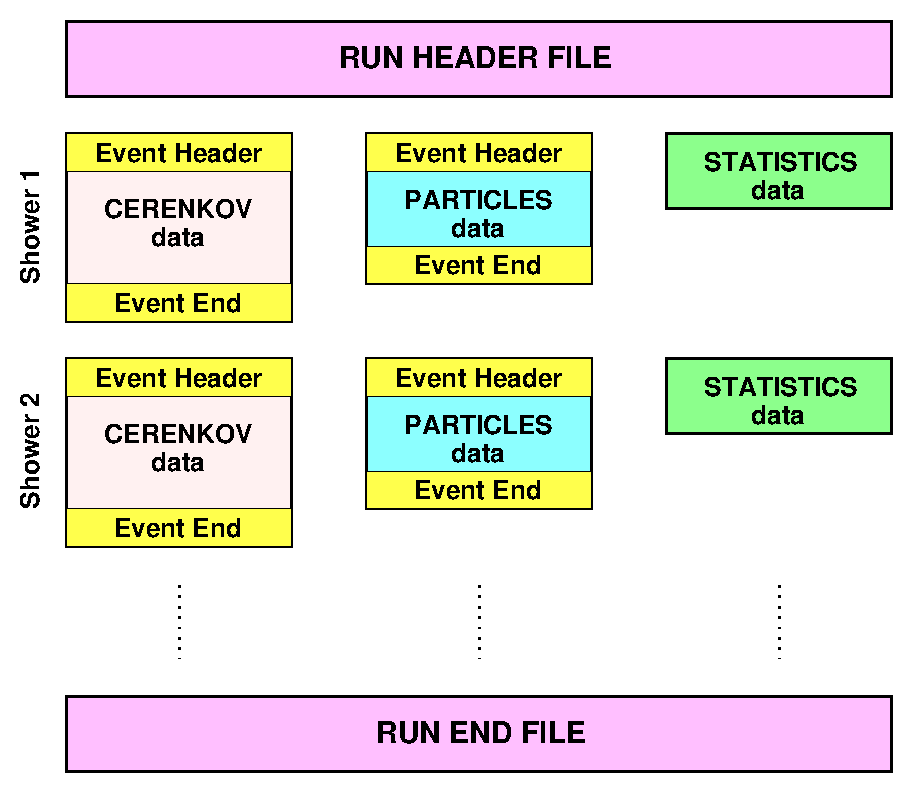
\epsfig{file=corsikastruc.eps,width=0.75\textwidth}
    \caption{Structure of the \CORSIKA output.}
    \label{fig:corsikastruc} 
  \end{center} 
\end{figure}
}

%%%%%%%%%%%%%%%%%%%%%%%%%%%%%%%%%%%%%%%%%%%%%%%%%%%%%%%%%%%%
\def\CORSIKAtableRH{
\begin{table}[p]
  \begin{center}
    \footnotesize
    \begin{tabular}{|r|l|}
\multicolumn{2}{c}{\bfseries Run header sub-block: (once per run)}\\
\hline
No. of word&Contents of word\\
\hline %%----------------------------------------
\hline %%----------------------------------------
1& `RUNH' \\
2& run number \\
3& date of begin run ( yymmdd ) \\
4&version of program \\
5& number of observation levels (maximum 10) \\
5+ $i$& height of level $i$ in cm\\
16 &slope of energy spectrum \\
17 &lower limit of energy range \\
18 &upper limit of energy range \\
19 &flag for EGS4 treatment of em. component \\
20 &flag for NKG treatment of em. component \\
21 &kin. energy cuto, for hadrons in GeV \\
22 &kin. energy cuto, for muons in GeV \\
23 &kin. energy cuto, for electrons in GeV \\
24 &energy cuto, for photons in GeV\\
\hline
\multicolumn{2}{|c|}{physical constants and interaction flags}\\
\hline
24+$i$ &C($i$), $i$ = 1,50 \\
74+$i$ &CC($i$), $i$ = 1,20 \\
94+$i$ &CKA($i$), $i$ = 1,40 \\
134+$i$& CETA($i$), $i$ = 1,5 \\
139+$i$& CSTRBA($i$),i = 1,11 \\
150+$i$& 0, $i$ = 1,4 (no longer used) \\
154+$i$& CAN($i$), $i$ = 1,50 \\
204+$i$& CANN($i$), $i$ = 1,50 \\
254+$i$& AATM($i$), $i$ = 1,5 \\
259+$i$& BATM($i$), $i$ = 1,5 \\
264+$i$& CATM($i$), $i$ = 1,5\\
270& NFLAIN (as real) \\
271& NFLDIF (as real) \\
272& NFLPI0+100$\times$NFLPIF (as real) \\
273& NFLCHE+100$\times$NFRAGM (as real)\\
\hline
    \end{tabular}
  \end{center}
  \caption{Structure of the run header sub-block}
  \label{tab:rh}
\end{table}
}

%%%%%%%%%%%%%%%%%%%%%%%%%%%%%%%%%%%%%%%%%%%%%%%%%%%%%%%%%%%%
\def\CORSIKAtableEHone{
\begin{table}[p]
  \begin{center}
    \footnotesize
    \begin{tabular}{|r|l|}
\multicolumn{2}{c}{\bfseries Event header sub-block: (once per event)}\\
\hline
No. of word&Contents of word\\
\hline %%----------------------------------------
\hline %%----------------------------------------
1& `EVTH'  \\
2& event number  \\
3& particle id (particle code or A$\times$ 100+Z for nuclei)  \\
4& total energy in GeV  \\
5& starting altitude in g=cm2  \\
6& number of first target if fixed  \\
7& z coordinate (height) of first interaction in cm  \\
8& px momentum in x direction in GeV  \\
9& py momentum in y direction in GeV  \\
10& pz momentum in -z direction in GeV \\
&(pz is positive for downward going particles)  \\
11& zenith angle $\theta$ in radian  \\
12& azimuth angle $\phi$ in radian  \\
13& number of different random number sequences (max. 10)  \\
11+3$\times$ $i$& integer seed of sequence $i$  \\
12+3$\times$ $i$& number of offset random calls ($\mathrm{mod} 10^6$) of sequence $i$  \\
13+3$\times$ $i$& number of offset random calls ($/10^6$) of sequence i \\
44& run number  \\
45& date of begin run (yymmdd)  \\
46& version of program  \\
47& number of observation levels  \\
47+$i$& height of level $i$ in cm \\
58& slope of energy spectrum  \\
59& lower limit of energy range in GeV  \\
60& upper limit of energy range in GeV  \\
61& cutoff for hadrons kinetic energy in GeV  \\
62& cutoff for muons kinetic energy in GeV  \\
63& cutoff for electrons kinetic energy in GeV  \\
64& cutoff for photons energy in GeV  \\
65& NFLAIN as a real number  \\
66& NFLDIF as a real number  \\
67& NFLPI0 as a real number  \\
68& NFLPIF as a real number  \\
69& NFLCHE as a real number  \\
70& NFRAGM as a real number  \\
71& x component of Earth's magnetic field in $\mu$T  \\
72& z component of Earth's magnetic field in $\mu$T  \\
73& flag for activating EGS4 as real number  \\
74& flag for activating NKG as real number \\
\hline
    \end{tabular}
  \end{center}
  \caption{Structure of event header sub-block.}
  \label{tab:eh1}
\end{table}
}

%%%%%%%%%%%%%%%%%%%%%%%%%%%%%%%%%%%%%%%%%%%%%%%%%%%%%%%%%%%%
\def\CORSIKAtableEHtwo{
\begin{table}[p]
  \begin{center}
    \footnotesize
    \begin{tabular}{|r|l|}
\multicolumn{2}{c}{\bfseries Event header sub-block: (continued)}\\
\hline
No. of word&Contents of word\\
\hline %%----------------------------------------
\hline %%----------------------------------------
75 &GHEISHA flag as real number                               \\
76 &VENUS flag as real number                                  \\
77 &CERENKOV flag as real number                               \\
78 &NEUTRINO flag as real number                               \\
79 &HORIZONT flag as real number                               \\
80 &computer flag (1=IBM, 2=Transputer, 3=DEC/UNIX,                              \\
&4=Macintosh, 5=VAX/VMS, 6=LINUX) as real number                               \\
81 &lower edge of $\theta$ interval (in $^\circ$)                               \\
82 &upper edge of $\theta$ interval (in $^\circ$)                               \\
83 &lower edge of OE interval (in $^\circ$)                               \\
84 &upper edge of OE interval (in $^\circ$)                               \\
85 &Cherenkov bunch size in the case of Cherenkov calculations                               \\
86 &number of Cherenkov detectors in x-direction                               \\
87 &number of Cherenkov detectors in y-direction                               \\
88 &grid spacing of Cherenkov detectors in x-direction in cm                               \\
89 &grid spacing of Cherenkov detectors in y-direction in cm                               \\
90 &length of each Cherenkov detector in x-direction in cm                               \\
91 &length of each Cherenkov detector in y-direction in cm                               \\
92 &Cherenkov output directed to particle output file (= 0.)                              \\
&or Cherenkov output file (= 1.)                                     \\
93 &angle (in rad) between array x-direction and magnetic north                               \\
94 &flag for additional muon information on particle output file                               \\
95 &step length factor for multiple scattering step length in EGS                               \\
96 &Cherenkov bandwidth lower end in nm \\
97 &Cherenkov bandwidth upper end in nm \\
98 &number $i$ of uses of each event \\
98+$i$& x coordinate of $i^{\mathrm{th}}$ core location for scattered events in cm \\
118+$i$& y coordinate of $i^{\mathrm{th}}$ core location for scattered events in cm\\
139 &SIBYLL interaction flag as real number \\
140 &SIBYLL cross section flag as real number \\
141 &QGSJET interaction flag as real number \\
142 &QGSJET cross section flag as real number \\
143 &DPMJET interaction flag as real number \\
144 &DPMJET cross section flag as real number \\
145 &VENUS cross section flag as real number \\
146 &muon multiple scattering flag (1.=Moli\`ere, 0.=Gauss) \\
147 &EFRCTHN energy fraction of thinning level \\
148 &NKG radial distribution range in cm \\
149...273 &not used\\
\hline
    \end{tabular}
  \end{center}
  \caption{Structure of event header sub-block (continued).}
  \label{tab:eh2}
\end{table}
}

%%%%%%%%%%%%%%%%%%%%%%%%%%%%%%%%%%%%%%%%%%%%%%%%%%%%%%%%%%%%
\def\CORSIKAtableEE{
\begin{table}[p]
  \begin{center}
    \footnotesize
    \begin{tabular}{|r|l|}
\multicolumn{2}{c}{\bfseries Event end sub-block}\\
\hline
No. of word&Contents of word\\
\hline %%----------------------------------------
\hline %%----------------------------------------
1 &`EVTE'  \\
2 &event number \\
&statistics for one shower :  \\
3 &weighted number of photons written to particle output file  \\
4 &weighted number of electrons written to particle output file  \\
5 &weighted number of hadrons written to particle output file  \\
6 &weighted number of muons written to particle output file  \\
7 &number of weighted particles written to particle output file PATAPE \\
&(This number includes also Cherenkov bunches, if Cherenkov output  \\
&is directed to PATAPE, but excludes additional muon information)  \\
&NKG output (if selected) :  \\
7+$i$&$i$= 1..21 lateral distribution in x direction for 1. level in \u{cm^2}\\  
28+$i$&$i$= 1..21 lateral distribution in y direction for 1. level in \u{cm^2}\\ 
49+$i$&$i$= 1..21 lateral distribution in xy direction for 1. level in \u{cm^2}\\
70+$i$&$i$= 1..21 lateral distribution in yx direction for 1. level in \u{cm^2}\\ 
91+$i$&$i$= 1..21 lateral distribution in x direction for 2. level in \u{cm^2}\\  
112+$i$&$i$= 1..21 lateral distribution in y direction for 2. level in \u{cm^2}\\ 
133+$i$&$i$= 1..21 lateral distribution in xy direction for 2. level in \u{cm^2}\\
154+$i$&$i$= 1..21 lateral distribution in yx direction for 2. level in \u{cm^2}\\
175+$i$&$i$= 1..10 electron number in steps of 100 \u{g/cm^2} \\ 
185+$i$&$i$= 1..10 age in steps of 100 \u{g/cm^2} \\ 
195+$i$&$i$= 1..10 distances for electron distribution in cm \\ 
205+$i$&$i$= 1..10 local age 1. level\\ 
215+$i$&$i$= 1..10 height of levels for electron numbers in \u{g/cm^2}\\  
225+$i$&$i$= 1..10 height of levels for electron numbers in cm \\ 
235+$i$&$i$= 1..10 distance bins for local age in cm \\ 
245+$i$&$i$= 1..10 local age 2. level \\ 
255+$i$&$i$= 1..6 parameters of longitudinal distribution of charged particles\\ 
262&$\chi^2$ per degree of freedom of fit to longitudinal distribution  \\
263..273&not used \\
\hline
    \end{tabular}
  \end{center}
  \caption{Structure of event end sub-block.}
  \label{tab:ee}
\end{table}
}

%%%%%%%%%%%%%%%%%%%%%%%%%%%%%%%%%%%%%%%%%%%%%%%%%%%%%%%%%%%%
\def\CORSIKAtableRE{
\begin{table}[p]
  \begin{center}
    \footnotesize
    \begin{tabular}{|r|l|}
\multicolumn{2}{c}{\bfseries Run end sub-block}\\
\hline
No. of word&Contents of word\\
\hline %%----------------------------------------
\hline %%----------------------------------------
1&`RUNE' \\
2&run number \\
3&number of events processed \\
4..273&not used yet\\
\hline
    \end{tabular}
  \end{center}
  \caption{Structure of run end sub-block.}
  \label{tab:re}
\end{table}
}

%%%%%%%%%%%%%%%%%%%%%%%%%%%%%%%%%%%%%%%%%%%%%%%%%%%%%%%%%%%%
\def\CORSIKAtablePART{
\begin{table}[p]
  \begin{center}
    \footnotesize
    \begin{tabular}{|r|l|}
\multicolumn{2}{c}{\bfseries Particle data sub-block : (up to 39 particles, 7 words each)}\\
\hline
No. of word&Contents of word \\
\hline %%----------------------------------------
\hline %%----------------------------------------
$7\times (n-1)+1$ &particle description \\
  &(part. id$\times$1000+ hadr. generation$\times$10+ no. of obs. level)  \\
$7\times (n-1)+2$ &px, momentum in x direction in GeV  \\
$7\times (n-1)+3$ &py, momentum in y direction in GeV  \\
$7\times (n-1)+4$ &pz, momentum in -z direction in GeV  \\
$7\times (n-1)+5$ &x coordinate in cm  \\
$7\times (n-1)+6$ &y coordinate in cm  \\
$7\times (n-1)+7$ &t time since first interaction in nsec \\
&(z coordinate in cm for additional muon information)  \\
\hline
\multicolumn{2}{|c|}{for n = 1 \ldots 39}\\
\multicolumn{2}{|c|}{last block may not be completely filled}\\
\hline
    \end{tabular}
  \end{center}
  \caption{Structure of particle data sub-block.}
  \label{tab:part}
\end{table}
}

%%%%%%%%%%%%%%%%%%%%%%%%%%%%%%%%%%%%%%%%%%%%%%%%%%%%%%%%%%%%
\def\CORSIKAtableCHER{
\begin{table}[p]
  \begin{center}
    \footnotesize
    \begin{tabular}{|r|l|}
\multicolumn{2}{c}{\bfseries Cherenkov photon data sub-block : (up to 39 photons, 7 words each)}\\
\hline
No. of word&Contents of word \\
\hline %%----------------------------------------
\hline %%----------------------------------------
$7\times (n-1)+1$ &j$\times$100000.+$\lambda$ \\
$7\times (n-1)+2$ &x coordinate in the obs.level, in cm\\
$7\times (n-1)+3$ &y coordinate in the obs.level, in cm\\
$7\times (n-1)+4$ &u direction cosine to x axis\\
$7\times (n-1)+5$ &v direction cosine to y axis\\
$7\times (n-1)+6$ &arrival time since first interaction in nsec\\
$7\times (n-1)+7$ &height of production of photon in cm\\
\hline
\multicolumn{2}{|c|}{for n = 1 \ldots 39}\\
\multicolumn{2}{|c|}{last block may not be completely filled}\\
\hline
    \end{tabular}
  \end{center}
  \caption{Structure of Cherenkov photon data sub-block. The value of 
    $j$ is defined as $j\equiv$number of the telescope which gave
    trigger (usually 1). We simulate with a bunch size (number of
    photons per sub-block) equal to 1.}
  \label{tab:cher}
\end{table}
}

%%%%%%%%%%%%%%%%%%%%%%%%%%%%%%%%%%%%%%%%%%%%%%%%%%%%%%%%%%%%
\def\CORSIKAtableSTA{
\begin{table}[p]
  \begin{center}
    \footnotesize
    \begin{tabular}{|r|l|}
\multicolumn{2}{c}{\bfseries Statistics data block}\\
\hline
No. of word&Contents of word \\
\hline %%----------------------------------------
\hline %%----------------------------------------
  1 \ldots 273 (273)& Event Header for this shower\\
274 \ldots 547 (273)&Event End for this shower\\
\hline
548&Time of the first photon stored in tape\\
549&Time of the last photon stored in tape\\
\hline
\multicolumn{2}{|c|}{for $i$ = 0 \ldots 9 $\longrightarrow$ 10 obs.levels}\\
\hline
550+$i\times 22$&Number of protons at obs.level $i$ \\
551+$i\times 22$&Number of antiprotons at obs.level $i$ \\
552+$i\times 22$&Number of neutrons at obs.level $i$ \\
553+$i\times 22$&Number of antineutrons at obs.level $i$ \\
554+$i\times 22$&Number of photons at obs.level $i$ \\
555+$i\times 22$&Number of electrons at obs.level $i$ \\
556+$i\times 22$&Number of positrons at obs.level $i$ \\
557+$i\times 22$&Number of neutrinos at obs.level $i$ \\
558+$i\times 22$&Number of $\mu^-$ at obs.level $i$ \\
559+$i\times 22$&Number of $\mu^+$ at obs.level $i$ \\
560+$i\times 22$&Number of $\pi^0$ at obs.level $i$ \\
561+$i\times 22$&Number of $\pi^-$ at obs.level $i$ \\
562+$i\times 22$&Number of $\pi^+$ at obs.level $i$ \\
563+$i\times 22$&Number of $K^0$ Long at obs.level $i$ \\
564+$i\times 22$&Number of $K^0$ Short  at obs.level $i$ \\
565+$i\times 22$&Number of $K^{*-}$  at obs.level $i$ \\
566+$i\times 22$&Number of $K^{*+}$  at obs.level $i$ \\
567+$i\times 22$&Number of strange Baryons at obs.level $i$ \\
568+$i\times 22$&Number of Deuterons at obs.level $i$ \\
579+$i\times 22$&Number of Tritons at obs.level $i$ \\
570+$i\times 22$&Number of $\alpha$ particles at obs.level $i$ \\
571+$i\times 22$&Number of other (strange) particles at obs.level $i$ \\
\hline
770&Number of Nucleons\\
771&Number of Pions   \\
772&Number of Etas    \\
773&Number of Kaons   \\
773&Number of strange Baryons\\
774&Number of Cherenkov photons from Electrons\\
775&Number of Cherenkov photons from Electrons\\
\hline
776&LPCT1 = 1 if Long.Distribution must be calculated\\
777&$N_{\mathrm{STEP}}$: Number of steps in the  Long.Distribution\\
778&$W_{\mathrm{STEP}}$: Width of the step in the  Long.Distribution\\
\hline
\multicolumn{2}{|c|}{\underline{\itshape Longitudinal distributions}}\\
\multicolumn{2}{|c|}{for $k$ = 0 \ldots 8 $\longrightarrow$ 9 species}\\
\multicolumn{2}{|c|}{$\gamma$,e$^+$,e$^-$,$\mu^-$,$\mu^+$,hadrons,charged
particles,nuclei and Cherenkov photons}\\
\multicolumn{2}{|c|}{and for $i$ = 0 \ldots $N_{\mathrm{STEP}}$}\\
\multicolumn{2}{|c|}{ $\longrightarrow$ $N_{\mathrm{STEP}}$ steps 
of $W_{\mathrm{STEP}}$}\\
\hline
779+$k\times N_{\mathrm{STEP}}+i$&Number of particles of specie
$k$ at depth $i\times W_{\mathrm{STEP}}$ g/cm$^2$ \\
\hline
    \end{tabular}
  \end{center}
  \caption{Structure of Statistics data block as saved in the
    \texttt{staXXXXXX} files.}
  \label{tab:sta}
\end{table}
}

%%%%%%%%%%%%%%%%%%%%%%%%%%%%%%%%%%%%%%%%%%%%%%%%%%%%%%%%%%%%
%% BEGIN DOCUMENT
%%%%%%%%%%%%%%%%%%%%%%%%%%%%%%%%%%%%%%%%%%%%%%%%%%%%%%%%%%%%
\begin{document}

%%%%%%%%%%%%%%%%%%%%%%%%%%%%%%%%%%%%%%%%%%%%%%%%%%%%%%%%%%%%
%% Please, for the formatting just include here the standard
%% elements: title, author, date, plus TDAScode
%%%%%%%%%%%%%%%%%%%%%%%%%%%%%%%%%%%%%%%%%%%%%%%%%%%%%%%%%%%%
\title{A short description of the data formats \\
involved in the MC simulation (I).\\
{\slshape The \CORSIKA and \texttt{reflector} output formats}}
\author{J C Gonz\'alez\\
Max Planck Institute for Physics, Munich\\ 
\texttt{<gonzalez@mppmu.mpg.de>}}
\date{July 10, 2000}
\TDAScode{MAGIC-TDAS 00-XX\\ 000710/JCGonzalez}
%%%%%%%%%%%%%%%%%%%%%%%%%%%%%%%%%%%%%%%%%%%%%%%%%%%%%%%%%%%%

%% title %%%%%%%%%%%%%%%%%%%%%%%%%%%%%%%%%%%%%%%%%%%%%%%%%%%%
\maketitle

%% abstract %%%%%%%%%%%%%%%%%%%%%%%%%%%%%%%%%%%%%%%%%%%%%%%%%
\begin{abstract}
  In this document I will try to explain a little bit the output
  format of the programs \CORSIKA version X.XX and \texttt{reflector}
  version X.XX. These formats are the ones which are used in the MAGIC
  Software Repository at the date of writing this small memo.\\
\end{abstract}

%% contents %%%%%%%%%%%%%%%%%%%%%%%%%%%%%%%%%%%%%%%%%%%%%%%%%
\thetableofcontents

\newpage

%% body %%%%%%%%%%%%%%%%%%%%%%%%%%%%%%%%%%%%%%%%%%%%%%%%%%%%%

%\chapter{Simulation of atmospheric showers}
\label{chapter:simshowers}

Usually, the \MC simulations of atmospheric showers follow a well
defined scheme. They start the simulation at the top of the
atmosphere, with a given primary particle. From there they simulate
the fly and interactions of this particle with its environment. At a
certain moment, this particle produces some secondary particles, which
are written to a stack, being processed each of them afterwards. Each
secondary particle have a certain probability of interact or decay,
and in virtue of this probability new (tertiary) particles are
produced and written into a new stack. The process follows until a
detector (or ground) is reached. See Fig. \ref{fig:MCsimGaisser} as an
example.

\mcsimsample

Several cuts (in energy, for example) or simplifications are normally
taken into account in the simulation programs in order to minimize the
computation time. The simulation code will reject, during the
simulation, those particles which fall into a ``dead zone'' of the
phase space of the parameters of the simulation, or of the detector.
For instance, if we are interested in detecting electrons, and our
instrument do only detect those above a sharp cut-off energy
$E_{\mathrm{threshold}}$, quite likely we are interested in removing
from the simulation process any electron as soon as he reaches this
energy.

%%==========================================================
\section{The \CORSIKA code}
\label{sec:CORSIKA}
%
One of the most spreadly used simulation codes in the field of cosmic
and $\gamma$-rays is the \CORSIKA code \cite{CORSIKA:manual}. The last
official version released at the time of writing this work is
\lastCORSIKA.  \CORSIKA (COsmic Ray SImulations for KAscade) is a
detailed Monte Carlo program to study the evolution and properties of
extensive air showers in the atmosphere, and was developed to perform
simulations for the KASKADE experiment, in Karlsruhe (Germany)
\cite{KASKADE} (this experiment aims to measure the elemental
composition of the primary cosmic radiation in the energy range
$3\E{14}$--$5\E{16}$\u{eV}). The code is mostly written in Fortran 77
(some pieces of code in new versions are written in C for portability)
and hence is easily portable to almost any computer.

\CORSIKA simulates interactions and decays of nuclei and subatomic
particles (hadrons, muons, electrons, photons, \ldots) up to energies
of 10\pow{17}\u{eV}. All secondary particles are tracked along their
trajectories and their parameters when reaching the user-defined
detector levels (energy, position, direction and arrival time) are
saved into disk.

\CORSIKA was originally developed on the basis of three well
established program systems. The first treats the hadronic part of
proton induced showers using the \emph{fire ball} and \emph{isobar},
and was written in the 70's by P.K.F. Grieder \cite{Grieder:1979}.
Nowadays, its structure serves as the general frame where \CORSIKA
handles its input and output, and the interaction routines used in
this program can be used as hadronic interactions at low energies. The
second program was developed by J.N. Capdevielle
\cite{Capdevielle:1989} following the \emph{Dual Parton Model}
(DPM)\cite{Capella:1980}, describing the interactions of protons at
high energies in good agreement with the measured collider data. The
third part, used for the simulation of the electromagnetic part of the
air shower, is based in the EGS4 code \cite{EGS4}. Whenever possible,
experimentally accesible data have been used.

For the simulation of the hadronic interactions several models can be
used (they are chosed by the user). The current available models are:

\begin{description}
  
\item[The DPM] These routines are based on the \emph{Dual Parton Model}
  and can be used for high energies to reproduce the kinematical
  distributions being measured or predicted by theory.
  
\item[VENUS] It simulates the inelastion ultra-relativistic heavy ion
  collisions with detailed simulation of creation, interaction and
  fragmentation of colour strings. It's the alternative to the DPM.
  
\item[Isobar and Fire-ball model routines] For low energy interactions
  
\item[GHEISHA] It's a more sophisticated replacement of the isobar and
  fire-ball routines. Suitable for energies up to several hundred
  \u{GeV}.

\item[Q??]      ??

\item[SYBILL] ??

\end{description}

The photoproduction of muon pairs and hadrons is added to the
electromagnetic part to allow the calculation of the muon content of
photon induced showers. A second way of treating the electromagnetic
component is to use the corrected and adapted form of the analytic NKG
formula for each electron or photon produced in the cascade.

It is also possible to include the generation of \Cherenkov light in
the atmosphere, to handle electronic and muonic neutrinos and
anti-neutrinos, and to simulate showers under nearly horizontal
incident directions (without the possibility of \Cherenkov light
generation, though).

We used a modified version of \CORSIKA 4.50, suitable for our purposes.
We modified the detector geometry in order to allow the simulation of
collection of light by \Cherenkov telescopes. Several minor
modifications were also introduced in order to make easier the
handling of the output data.

\subsection{Input and output from \CORSIKA}
%
The input for a \CORSIKA run is a plain ASCII parameters file, with
several entries in the form ``\texttt{KEYWORD <par1> <par2>} \ldots'',
where \texttt{<parN>} means the N-th parameter for that keyword
\texttt{KEYWORD}. An example of a parameters file is shown in Fig.
\ref{fig:CORSIKAparamfile}.

\CORSIKAsampleInputfig

Among other parameters, the user can set the type of primary for the
showers (\texttt{PRMPAR}), the run number (\texttt{RUNNR}), the number
of event for this run (\texttt{NSHOW}), the energy range
(\texttt{ERANGE}), the simulated slope of the spectrum in this energy
range (\texttt{ESLOPE}), the range of $(\theta,\phi)$ angles
(\texttt{THETAP}, \texttt{PHIP}), the observation levels
(\texttt{OBSLEV}), the cuts in energy (\texttt{ECUTS}) which allow us
to reduce the computation time by rejecting those particles below a
certain threshold, and the geometry of the detector (\texttt{CERARY}
in the original version, \texttt{ERANGE} and \texttt{ERANGE} in our
modified version).

\CORSIKA is able to treat the particles that are listed in Table
\ref{table:CORSIKAGeantcodes}

\CORSIKAGeanttableA

\CORSIKAGeanttableB

The output of \CORSIKA comes in two different ways. First, we have an
ASCII output, with statistics and sumaries of the simulation of the
showers and even with debugging information if needed.  The real
output of \CORSIKA is given in binary format. For each particle hitting
the detector area in our pre-defined observation levels we get the
type of the particle, the position in the plane of that observation
level, the direction, the energy, the height of production and the
arrival time. If we selected the CERENKOV version of \CORSIKA, we'll be
able to get information about the \Cherenkov photons as well. Due to
the huge number of \Cherenkov photons produces at high energies, we
can generate and follow them in groups (\emph{bunches}).  However, for
our purposes we traced each single \Cherenkov photon. For these
photons we stored into disk the wavelength, the position, the
direction, height of production and arrival time.


\MORE%%%%%%%%%%%%%%%%%%%%%%%%%%%%%%%%%%%%%%%%%%%%%%%%%%%%%%%%%%%%

%%==========================================================
\section{Simulation of showers at High Zenith Angle}

%%==========================================================
\section{Information available from the showers}

%%==========================================================
\section{Time Structure of the \Cherenkov pulse from an atmospheric shower}

%%%%%%%%%%%%%%%%%%%%%%%%%%%%%%%%%%%%%%%%%%%%%%%%%%%%%%%%%%
\section{Other simulation methods}
\label{sec:simothers}

\section{\CORSIKA output data format}

The output or the currently used \CORSIKA code is structured as shown
in Fig. \ref{fig:corsikastruc}. For each run with $N$ showers we will
end up with $3 N+2$ binary data files, with information about the
run and each individual shower. These files are (in the following list
\texttt{XXXXXX} means a 6-digit number):

\CORSIKAstructfig

\begin{itemize}
  
\item A \emph{Run Header file}, \texttt{runXXXXXX}, with information
  about the whole run (see Table \ref{tab:rh}). It's the first data
  file generated.
  
\item A \emph{Run End file}, \texttt{endXXXXXX}, with information
  about the whole run and some statistics about the run just generated
  (see Table \ref{tab:re}). It's the last file generated. It's sole
  presence indicates that the run has been finished.
  
\item One \emph{Particle data file} per shower, \texttt{datXXXXXX},
  with information about the particles (not Cherenkov photons)
  generated in the shower and which arrived at the ground (actually,
  at any user defined obs. level), in the user-defined area (see Table
  \ref{tab:part}).
  
\item One \emph{Cherenkov data file} per shower, \texttt{cerXXXXXX},
  with information about the Cherenkov photons generated in the shower
  and which arrived at the ground (actually, at any user defined obs.
  level), in the user-defined area (see Table \ref{tab:cher}).
  
\item One \emph{Statistics data file} per shower, \texttt{staXXXXXX},
  with information longitudinal profiles for different showers and
  other parameters of the shower (see Table \ref{tab:sta}).

\end{itemize}

As you can see in Fig.\ref{fig:corsikastruc}, each Particle and
Cherenkov file has an \emph{Event Header}, a list of \emph{Particle}
or \emph{Cherenkov photon} data blocks, and an \emph{Event End}. The
information stored in the \emph{Event Header} and \emph{Event End}
data blocks are shown in Tables \ref{tab:eh1}-\ref{tab:eh2} and
\ref{tab:ee}.

The structure of each \emph{Particle} or \emph{Cherenkov photon}
sub-blocks is shown in Tables \ref{tab:part}-\ref{tab:cher}.

\CORSIKAtableRH

\CORSIKAtableRH

\CORSIKAtableEHone

\CORSIKAtableEHtwo

\CORSIKAtableEE

\CORSIKAtableRE

\CORSIKAtablePART

\CORSIKAtableCHER

\CORSIKAtableSTA{

%------------------------------------------------------------
\section{Input data structures for \reflector}

The input data for \reflector, apart from the human-readable ASCII
format for the parameters file\footnote{The format of the parameters
  file will be explained in a next revision of this document},
consists of the output files from \CORSIKA. The format of these output
files has been already presented in the previous section, and the data
stored inside each block has been shown in tables
\ref{tab:rh}--\ref{tab:sta}. These data are read by \reflector through
some classes, which internal data members are shown in tables
\ref{class:coreh}.

%\begin{Class}[p]
%  \begin{center}
%  \scriptsize
%  \end{center}
%  \caption{Data members in clas \texttt{COREventHeader} used by \reflector.}
%  \label{class:coreh}
%\end{Class}

\lstset{%
language=C++,%
basicstyle=\scriptsize\sffamily,%
keywordstyle=\bfseries,%
commentstyle=\rmfamily\itshape,%
stringstyle=\sffamily,%
%labelstyle=\tiny\itshape,%
%labelstep=10,%
indent=1em,%
tabsize=2}

\lstinputlisting[keywords={char,Float_t}]{COREventHeader.class}



%%% BIBLIOGRAPHY %%%%%%%%%%%%%%%%%%%%%%%%%%%%%%%%%%%%%%%%

%%>>>> Use the following if you are using BibTeX for bibliography
%\theBibliography

\end{document}
%
%%%%%%%%%%%%%%%%%%%%%%%%%%%%%%%%%%%%%%%%%%%%%%%%%%%%%%%%%%%%%%%%%%%%%%%%%%%%%
%%% Upper-case    A B C D E F G H I J K L M N O P Q R S T U V W X Y Z
%%% Lower-case    a b c d e f g h i j k l m n o p q r s t u v w x y z
%%% Digits        0 1 2 3 4 5 6 7 8 9
%%% Exclamation   !           Double quote "          Hash (number) #
%%% Dollar        $           Percent      %          Ampersand     &
%%% Acute accent  '           Left paren   (          Right paren   )
%%% Asterisk      *           Plus         +          Comma         ,
%%% Minus         -           Point        .          Solidus       /
%%% Colon         :           Semicolon    ;          Less than     <
%%% Equals        =           Greater than >          Question mark ?
%%% At            @           Left bracket [          Backslash     \
%%% Right bracket ]           Circumflex   ^          Underscore    _
%%% Grave accent  `           Left brace   {          Vertical bar  |
%%% Right brace   }           Tilde        ~
%%%%%%%%%%%%%%%%%%%%%%%%%%%%%%%%%%%%%%%%%%%%%%%%%%%%%%%%%%%%%%%%%%%%%%%%%%%%%
%% Local Variables:
%% mode:latex
%% mode:font-lock
%% mode:auto-fill
%% time-stamp-line-limit:100
%% End:
%% EOF
